\chapwithtoc{Results}
\label{res}

\secwithtoc{First set of physicochemical attributes}
\label{res:first}

	In this section, results for the first set of physicochemical properties described
	above will be presented.
	These include the length, iso-electric point, GRAVY index, and percentage of charged
	amino acids within the non-domain regions of human two-domain protein kinases containing
	one kinase domain.

	\subsecwithtoc{Densities}
	\label{res:first:dens}

		The density analysis gave interesting insights into the representation of
		physicochemical properties within the studied dataset.
		The linker length density peaks around 75 residues.
		A small portion of extremely long inter-domain regions spanning 500 to 800 residues is
		also present.
		However, it is questionable, whether these ``linkers'' might not represent an yet
		unrecognized domain, thus not being suitable for the definition of a
		linker~\cite{milano2016structural}.

		An nontrivial outcome has been observed while studying the density of linkers'
		iso-electric point, visualized in \cref{fig:iso-dens}.
		Most non-domain regions in human two-domain protein kinases are either very acidic, or
		on the other hand, very basic
		The region of neutral pH contains almost no proteins, forming an empty gap around pH
		8.
		This allows for dividing the studied protein kinases into two groups based on their
		linker's acidity.

		\begin{figure}
			\centering
			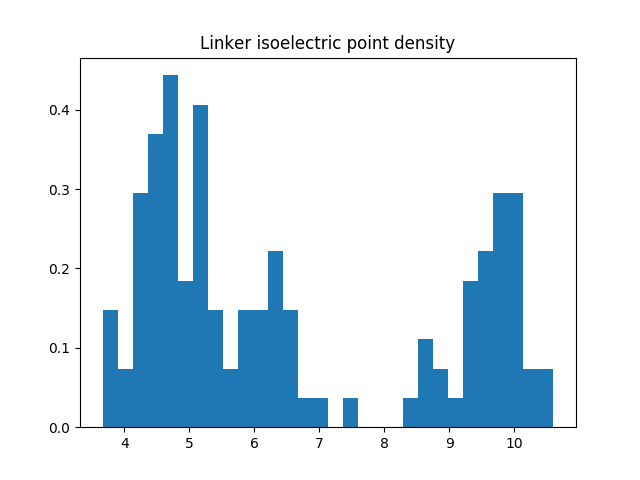
\includegraphics[width=.7\linewidth]{img/iso_density.png}
			\caption{The iso-electric point density of inter-domain regions from human
			two-domain protein kinases in the studied dataset. Two groups of proteins are
			evident, one with acidic linkers, one with basic linkers.}
			\label{fig:iso-dens}
		\end{figure}

		Au contraire, neither the percentage of charged amino acids within the non-domain
		regions, nor the linkers' GRAVY index, form distinct clusters.
		Their densities show only single local maxima.
		All linkers from the final dataset are hydrophilic, the percentage of charged residues
		averages around 0.25, hence not giving any surprising results.

	\subsecwithtoc{UMAP dimensionality reduction}
	\label{res:first:umap}

		Using the first set of linkers' physicochemical attributes, the clusters visible from
		the UMAP dimensionality reduction define three linker types.
		Throughout this thesis, the linker types will be referred to based on the clusters'
		positioning in \cref{fig:umap}: ``L-linkers'' for the lower left cluster,
		``M-linkers'' for the middle cluster, and ``R-linkers'' for the right cluster.
		L-linkers are best characterized by their extreme length of more than 600 residues,
		R-linkers by their extremely basic iso-electric point, and M-linkers by their
		extremely acidic iso-electric point, as well as by their GRAVY index being negatively
		proportional to their percentage of charged amino acids.

		\begin{figure}
			\centering
			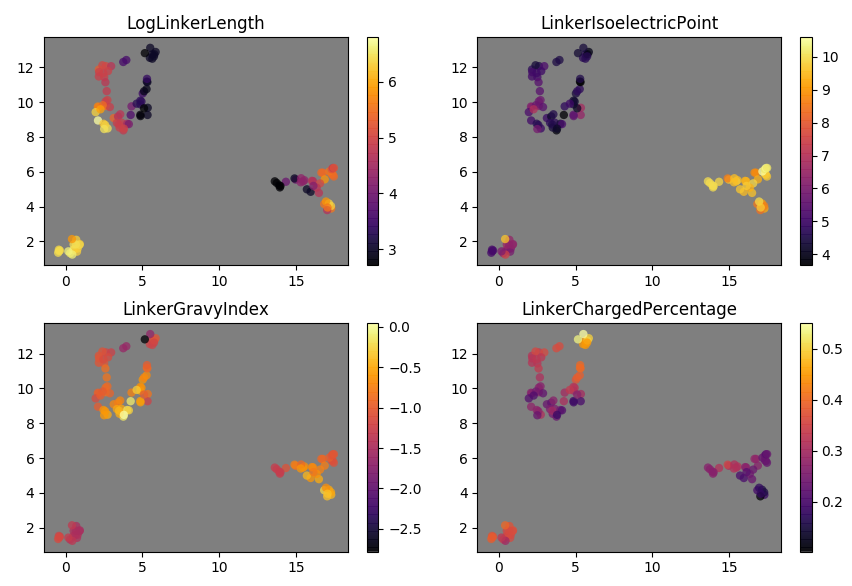
\includegraphics[width=\linewidth]{img/linker_umap.png}
			\caption{UMAP dimensionality reduction of the normalized linker attributes:
			logarithm of linker's length, iso-electric point, GRAVY index, and percentage of
			charged amino acids within the non-domain regions of human two-domain protein
			kinases. The values of the four physicochemical properties are embedded into the
			same UMAP representation, each subfigure corresponding to one attribute.}
			\label{fig:umap}
		\end{figure}

		\begin{figure}
			\centering
			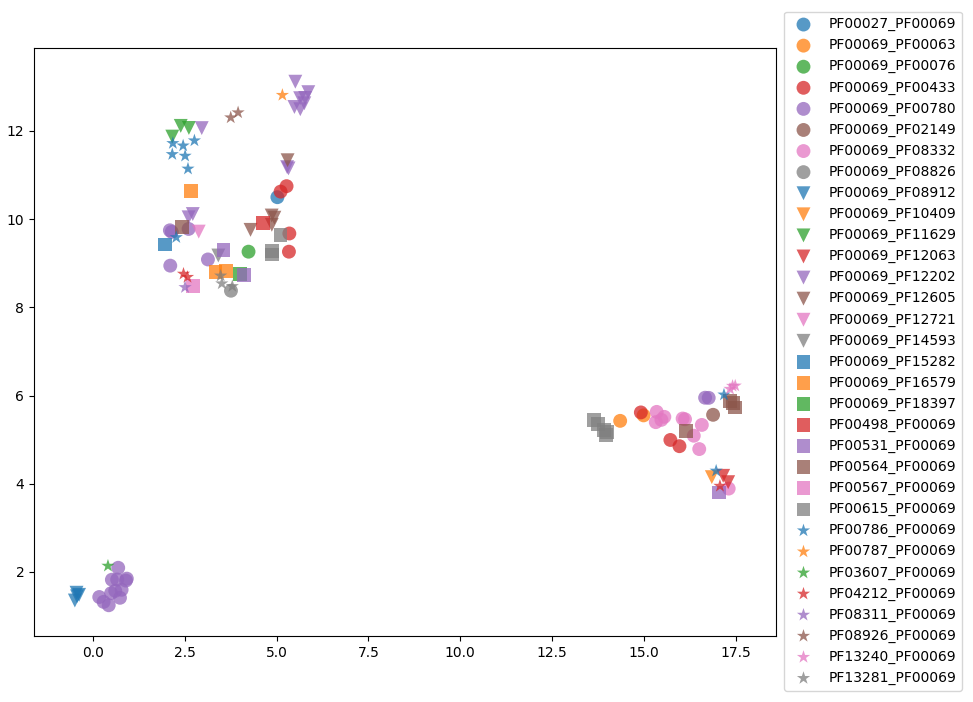
\includegraphics[width=0.9\linewidth]{img/linker_umap_arch.png}
			\caption{Architectures of the studied molecules embedded into the UMAP
			dimensionality reduction of four physicochemical attributes of non-domain regions.}
			\label{fig:umap_arch}
		\end{figure}

		By embedding the architectures of the proteins from the studied dataset into the UMAP
		representation, it is visible, that many architectures feature more than one linker
		type, as seen in \cref{fig:umap_arch}.
		Especially the architecture \texttt{PF00069\_PF00780} stands out, being endowed with
		all three linker classes.
		On the other hands, most architectures equipped with linkers from only one category
		are represented by a very narrow subset of proteins from the set of human two-domain
		protein kinases.

	\subsecwithtoc{Gene Ontology terms}
	\label{res:first:go}

		All considered proteins had at least two GO terms, one of them being always
		\texttt{GO:0005524; F:ATP binding}.
		The second most common was \texttt{GO:0004674; F:protein serine/threonine kinase
		activity}, and the third most frequent GO term was \texttt{GO:0004672; F:protein
		kinase activity}.

		However, the search for unique GO terms within both UMAP dimensionality reduction and
		iso-electric point clustering of the non-domain regions on different GO hierarchical
		levels gave no satisfactory results, albeit discovering many GO terms exclusive for
		each examined linker group.
		These terms were namely terribly underrepresented in proteins found within the
		clusters, and no unique vocable was found spanning any whole inter-domain region
		bundle.

		There were only two GO terms standing out, regarding their proportion.
		\texttt{GO:0000287; F:magnesium ion binding} found on hierarchy level 6 is exclusive
		to the acidic linker group, as well as to the M-linkers.
		It was encountered in 12 proteins, covering 8 different architectures, including those
		having the \texttt{PF00069} domain on the N-terminus, as well as those carrying the
		protein kinase domain on the C-terminus.
		The second vocable is \texttt{GO:0005516; F:calmodulin binding} appearing on hierarchy
		level 4, being limited to the basic linker group, likewise to the R-linkers.
		Regrettably, all 10 proteins accredited with this GO term possess the same
		architecture.

	\subsecwithtoc{Enzyme Commission numbers}
	\label{res:first:ec}

		\begin{figure}
			\centering
			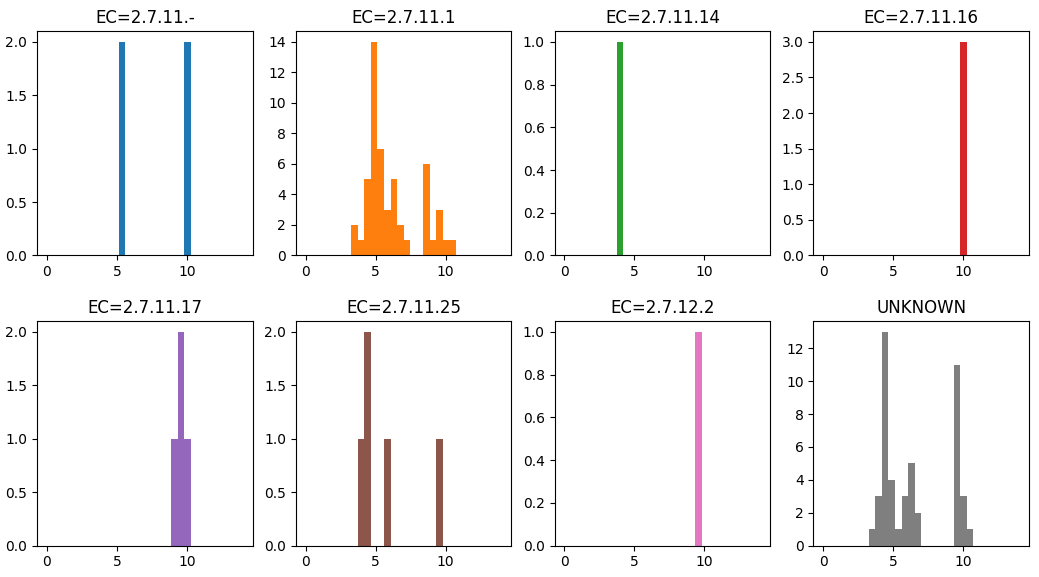
\includegraphics[width=\linewidth]{img/iso_density_ec.png}
			\caption{Occurrences of EC numbers in human two-domain protein kinases. The $x$-axis
			represents the iso-electric point of the molecules' linkers.}
			\label{fig:ec}
		\end{figure}

		Out of the 117 human two-domain protein kinases, 70 molecules have an EC number
		assigned in the \texttt{uniprot\_reference\_proteomes.dat} file.
		For the remaining 47, the Enzyme Commission term will be reffered to as
		``\texttt{UNKNOWN}''.
		3 kinases had more than one EC number specified, some of these extra terms are
		outside of the \texttt{2.7.11 protein-serine/threonine kinases} group.
		Only 14 molecules had, however, EC classification other than \texttt{2.7.11.-},
		\texttt{2.7.11.1 non-specific serine/threonine protein kinase}, or \texttt{UNKNOWN}.

		\Cref{fig:ec} shows the distribution of the linkers' iso-electric point for each EC
		number.
		All 5 specialized EC terms are vastly underrepresented within the studied dataset, yet
		for example the \texttt{2.7.11.25 mitogen-activated protein kinase kinase kinases}
		are even present in both acidic and basic linker cluster.
		Contrarily, basic inter-domain regions seem to be specific to both \texttt{2.7.11.16
		G-protein coupled receptor kinases} and
		\texttt{2.7.11.17 Ca\textsuperscript{2+}/calmodulin-dependent protein kinases},
		nevertheless, they are not to be found in more than one architecture.

		\begin{figure}
			\centering
			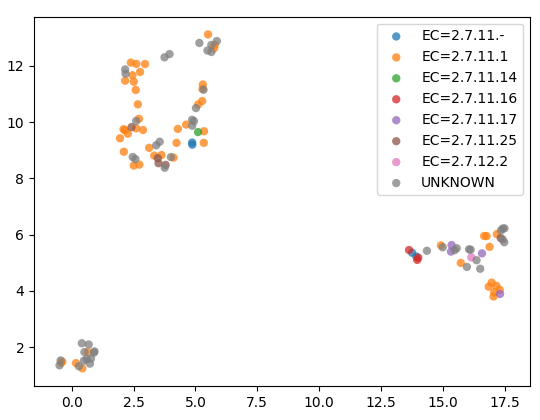
\includegraphics[width=0.8\linewidth]{img/linker_umap_ec.png}
			\caption{Embedding of the EC numbers into the UMAP dimensionality reduction
			visualization.}
			\label{fig:umap_ec}
		\end{figure}

		The inadequate representation of the EC numbers in the final dataset was also the
		reason behind the unsatisfactory results of embedding the terms into the UMAP
		dimensionality reduction.
		On one hand, the numbers \texttt{2.7.11.14}, \texttt{2.7.11.16}, and
		\texttt{2.7.11.17} are specific to one of the three defined linker groups, on the
		other hand, they are not to be found in more than one architecture, as already
		mentioned above.
		In conclusion, the first set of physicochemical attributes did not provide any
		interesting results.

\secwithtoc{Second set of physicochemical attributes}
\label{res:second}

	The UMAP dimensionality reduction of the 553 physicochemical data from the AAindex
	database did not reflect the clustering of 4 physicochemical attributes described above
	at all.
	As seen in \cref{fig:aa_umap}, one small cluster of non-domain regions from human
	two-domain protein kinases emerges on the right side of the visualization, however,
	it contains only proteins with the same architecture \texttt{PF00069\_PF12202}.
	In the large cloud on the left side, generally, molecules with the same architecture
	create local bundles, and they only seldom mix with proteins with other
	architectures.
	Due to the lack of clearly distinguishable clusters, no GO or EC embedding was
	performed.

	\begin{figure}
		\centering
		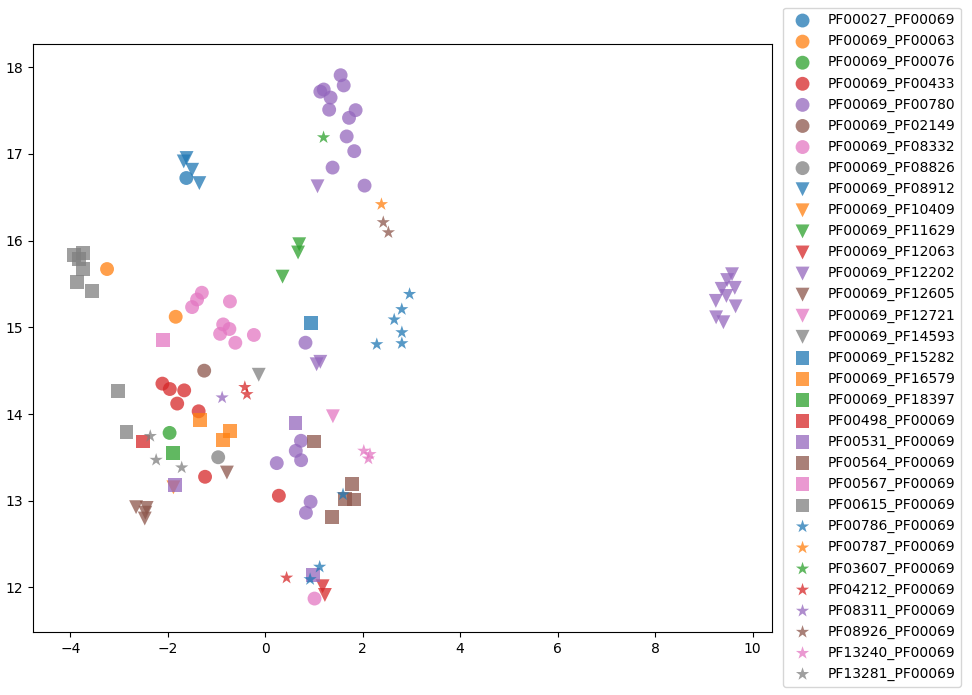
\includegraphics[width=0.9\linewidth]{img/aa_umap_arch.png}
		\caption{Architectures of the two-domain protein kinases with a single protein kinase
		domain embedded into the UMAP dimensionality reduction of 553 physicochemical
		properties from the AAindex database.}
		\label{fig:aa_umap}
	\end{figure}

	In conclusion, no obvious influence of non-domain regions' composition on the activity
	of human two-domain protein kinases with exactly one protein kinase domain was observed,
	as no evident clustering of the linkers' physicochemical properties segregating frequent
	GO terms or EC numbers belonging to different architectures was achieved.
